\section{Proof of concept system}\label{sec:poc_system_evaluation}

The proof of concept web-application is primarily responsible for performing two tasks.
\begin{itemize}
    \item{Given a product URL, extract the price history of the product and display it in a graphical format.}
    \item{Given a product URL, find similar products and display them in a tabular format.}
\end{itemize}

To measure the system's performance in these two tasks, a simple performance testing script was created to measure the time for the API to return the results for each of the two tasks.
The script works as follows:
\begin{enumerate}
    \item Retrieve a list of 1,000 product URLs from the database.
        \subitem The URLs are retrieved in such a way that there is an even distribution across all tracked domains.
    \item For each product URL, send a request to the API to retrieve the price history.
    \item Wait for a response from the API and record the time taken for the response to be received.
    \item For each product URL, send a request to the API to retrieve similar products.
    \item Wait for a response from the API and record the time taken for the response to be received.
    \item Graph the two response times and calculate the p50 and p95 response times for each of the two tasks.
\end{enumerate}

The above script makes each API call sequentially, which means that the next API call is made only after the previous API call has completed and a response has been received.
This may not reflect actual usage and behavior of the system, as in a real-world scenario, multiple users may be making requests to the API simultaneously.
However, for the purpose of this evaluation, the sequential API calls are sufficient to measure the performance of the system.
Figure~\ref{fig:poc_system_performance} shows the results of the two tasks, with the p50 and p95 response times for each task.

\begin{figure}[h]
    \centering
    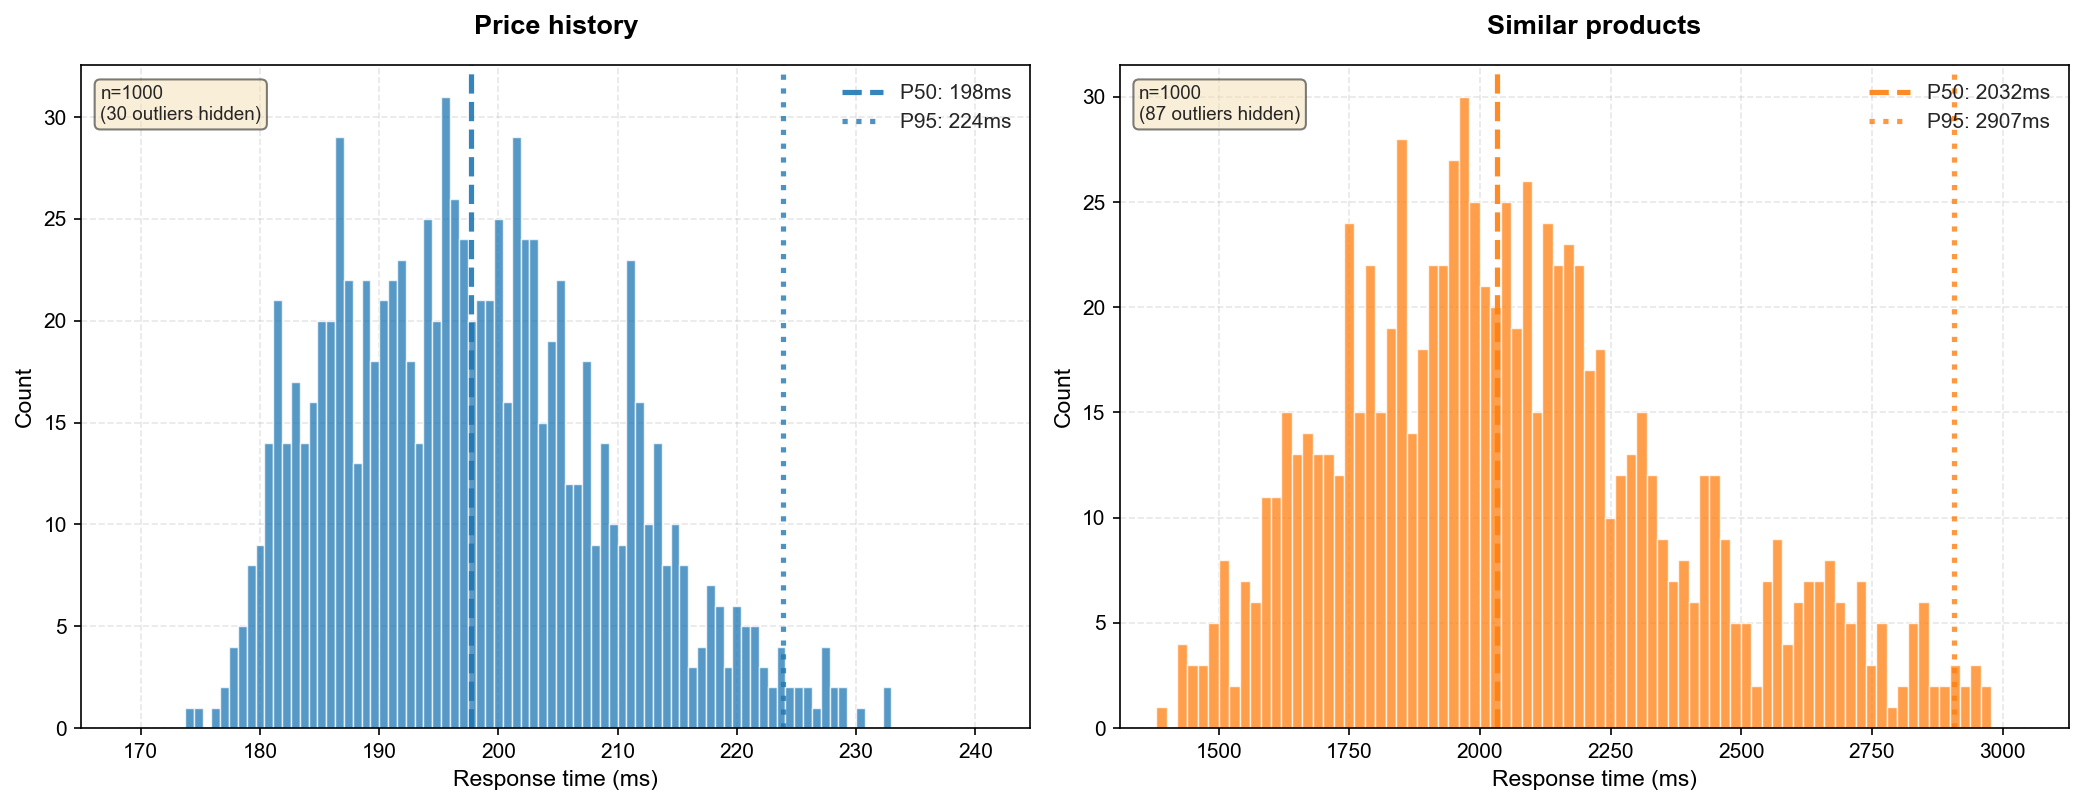
\includegraphics[width=1\textwidth]{images/poc_system_performance}
    \caption{Response time for the two tasks performed by the proof of concept system.}
    \label{fig:poc_system_performance}
\end{figure}

As can be seen from Figure~\ref{fig:poc_system_performance}, the \texttt{p50} response time for the price history task is \texttt{0.198} seconds, while the \texttt{p95} response time is \texttt{0.224} seconds.
For the similar products task, the \texttt{p50} response time is \texttt{2.032} seconds, while the \texttt{p95} response time is \texttt{2.907} seconds